\ifx\wholebook\relax \else
% ------------------------

\documentclass[UTF8]{article}
%------------------- Other types of document example ------------------------
%
%\documentclass[twocolumn]{IEEEtran-new}
%\documentclass[12pt,twoside,draft]{IEEEtran}
%\documentstyle[9pt,twocolumn,technote,twoside]{IEEEtran}
%
%-----------------------------------------------------------------------------
%
% loading packages
%

\RequirePackage{ifpdf}
\RequirePackage{ifxetex}

%
%
\ifpdf
  \RequirePackage[pdftex,%
       bookmarksnumbered,%
              colorlinks,%
          linkcolor=blue,%
              hyperindex,%
        plainpages=false,%
       pdfstartview=FitH]{hyperref}
\else\ifxetex
  \RequirePackage[bookmarksnumbered,%
               colorlinks,%
           linkcolor=blue,%
               hyperindex,%
         plainpages=false,%
        pdfstartview=FitH]{hyperref}
\else
  \RequirePackage[dvipdfm,%
        bookmarksnumbered,%
               colorlinks,%
           linkcolor=blue,%
               hyperindex,%
         plainpages=false,%
        pdfstartview=FitH]{hyperref}
\fi\fi
%\usepackage{hyperref}

% other packages
%--------------------------------------------------------------------------
\usepackage{graphicx, color}
\usepackage{subfig}
\usepackage{tikz}
\usetikzlibrary{matrix,positioning}

\usepackage{amsmath, amsthm, amssymb} % for math
\usepackage{exercise} % for exercise
\usepackage{import} % for nested input

%
% for programming
%
\usepackage{verbatim}
\usepackage{listings}
%\usepackage{algorithmic} %old version; we can use algorithmicx instead
%\usepackage[plain]{algorithm} %remove rule (horizontal line on top/below the algorithm
\usepackage{algorithm} %to remove rules change to \usepackage[plain]{algorithm}
%\usepackage{algorithm2e}
\usepackage[noend]{algpseudocode} %for pseudo code, include algorithmicsx automatically
\usepackage{appendix}
\usepackage{makeidx} % for index support
\usepackage{titlesec}

\usepackage[cm-default]{fontspec}
\usepackage{xunicode}
%\usepackage{fontenc}
\usepackage{textcomp}

% detect and select Chinese font
% ------------------------------
% the following cmd can list all availabe Chinese fonts in host.
% fc-list :lang=zh
\def\myfont{STSong}  % Under Mac OS X
\def\linuxfallback{WenQuanYi Micro Hei} % Under Linux
\def\winfallback{SimSun} % Under Windows
\suppressfontnotfounderror1 % Avoid setting exit code (error level) to break make process
\count255=\interactionmode
\batchmode
\font\foo="\myfont"\space at 10pt
\ifx\foo\nullfont
  \font\foo = "\linuxfallback"\space at 10pt
  \ifx\foo\nullfont
    \font\foo = "\winfallback"\space at 10pt
    \ifx\foo\nullfont
      \errorstopmode
      \errmessage{no suitable Chinese font found}
    \else
      \let\myfont=\winfallback % Windows
    \fi
  \else
    \let\myfont=\linuxfallback % Linux
  \fi
\fi
\interactionmode=\count255
\setmainfont[Mapping=tex-text]{\myfont}
\setmonofont{Monaco}   % 英文等宽字体

\XeTeXlinebreaklocale "zh"  % to solve the line breaking issue
\XeTeXlinebreakskip = 0pt plus 1pt minus 0.1pt

\titleformat{\paragraph}
{\normalfont\normalsize\bfseries}{\theparagraph}{1em}{}
\titlespacing*{\paragraph}
{0pt}{3.25ex plus 1ex minus .2ex}{1.5ex plus .2ex}

\lstdefinelanguage{Smalltalk}{
  morekeywords={self,super,true,false,nil,thisContext}, % This is overkill
  morestring=[d]',
  morecomment=[s]{"}{"},
  alsoletter={\#:},
  escapechar={!},
  literate=
    {BANG}{!}1
    {UNDERSCORE}{\_}1
    {\\st}{Smalltalk}9 % convenience -- in case \st occurs in code
    % {'}{{\textquotesingle}}1 % replaced by upquote=true in \lstset
    {_}{{$\leftarrow$}}1
    {>>>}{{\sep}}1
    {^}{{$\uparrow$}}1
    {~}{{$\sim$}}1
    {-}{{\sf -\hspace{-0.13em}-}}1  % the goal is to make - the same width as +
    %{+}{\raisebox{0.08ex}{+}}1		% and to raise + off the baseline to match -
    {-->}{{\quad$\longrightarrow$\quad}}3
	, % Don't forget the comma at the end!
  tabsize=2
}[keywords,comments,strings]

% for literate Haskell code
\lstdefinestyle{Haskell}{
  flexiblecolumns=false,
  basewidth={0.5em,0.45em},
  morecomment=[l]--,
  literate={+}{{$+$}}1 {/}{{$/$}}1 {*}{{$*$}}1 {=}{{$=$}}1
           {>}{{$>$}}1 {<}{{$<$}}1 {\\}{{$\lambda$}}1
           {\\\\}{{\char`\\\char`\\}}1
           {->}{{$\rightarrow$}}2 {>=}{{$\geq$}}2 {<-}{{$\leftarrow$}}2
           {<=}{{$\leq$}}2 {=>}{{$\Rightarrow$}}2
           {\ .}{{$\circ$}}2 {\ .\ }{{$\circ$}}2
           {>>}{{>>}}2 {>>=}{{>>=}}2
           {|}{{$\mid$}}1
}

\lstloadlanguages{C, C++, Lisp, Haskell, Python, Smalltalk}

\lstset{
  basicstyle=\small\ttfamily,
  commentstyle=\rmfamily,
  texcl=true,
  showstringspaces = false,
  upquote=true,
  flexiblecolumns=false
}

% ======================================================================

\def\BibTeX{{\rm B\kern-.05em{\sc i\kern-.025em b}\kern-.08em
    T\kern-.1667em\lower.7ex\hbox{E}\kern-.125emX}}

%
% mathematics
%
\newcommand{\be}{\begin{equation}}
\newcommand{\ee}{\end{equation}}
\newcommand{\bmat}[1]{\left( \begin{array}{#1} }
\newcommand{\emat}{\end{array} \right) }
\newcommand{\VEC}[1]{\mbox{\boldmath $#1$}}

% numbered equation array
\newcommand{\bea}{\begin{eqnarray}}
\newcommand{\eea}{\end{eqnarray}}

% equation array not numbered
\newcommand{\bean}{\begin{eqnarray*}}
\newcommand{\eean}{\end{eqnarray*}}

\newtheorem{theorem}{Theorem}[section]
\newtheorem{lemma}[theorem]{引理}
\newtheorem{proposition}[theorem]{Proposition}
\newtheorem{corollary}[theorem]{Corollary}

% 中文书籍设置
% ====================================
\renewcommand\contentsname{目\ 录}
%\renewcommand\listfigurename{插图目录}
%\renewcommand\listtablename{表格目录}
\renewcommand\figurename{图}
\renewcommand\tablename{表}
\renewcommand\proofname{证明}
\renewcommand\ExerciseName{练习}
%\renewcommand{\algorithmcfname}{算法}

\ifx\wholebook\relax
\renewcommand\bibname{参\ 考\ 文\ 献}                    %book类型
%\newtheorem{Definition}[Theorem]{定义}
\newtheorem{Theorem}{定理}[chapter]
\newtheorem{example}{例题}[chapter]
\else
\renewcommand\refname{参\ 考\ 文\ 献}
\fi

%\setcounter{secnumdepth}{4}
\titleformat{\chapter}
  {\normalfont\bfseries\Large}
  {第\arabic{chapter}章}
  {12pt}{\Large}
%% \titleformat{\subsection}
%%   {\normalfont\bfseries\large}
%%   {\CJKnumber{\arabic{subsection}}、}
%%   {12pt}{\large}
%% \titleformat{\subsubsection}
%%   {\normalfont\bfseries\normalsize}
%%   {\arabic{subsubsection}.}
%%   {12pt}{\normalsize}

%\renewcommand{\baselinestretch}{1.5}                        %文章行间距为1.5倍。

\setcounter{tocdepth}{4}
\setcounter{secnumdepth}{4}


\setcounter{page}{1}

\begin{document}

%--------------------------

% ================================================================
%                 COVER PAGE
% ================================================================

\title{并不简单的队列}

\author{刘新宇
\thanks{{\bfseries 刘新宇 } \newline
  Email: liuxinyu95@gmail.com \newline}
  }

\maketitle
\fi

\markboth{队列}{初等算法}

\ifx\wholebook\relax
\chapter{并不简单的队列}
\numberwithin{Exercise}{chapter}
\fi

% ================================================================
%                 Introduction
% ================================================================
\section{简介}
\label{introduction}

队列是一种看起来比较简单的数据结构。它提供了FIFO(先进先出)处理数据的机制。有多种方法可以实现队列,包括使用单向或双向链表,使用循环buffer等。但是,在满足队列性质的条件下(尤其式性能限制条件),实现一个纯函数式队列却并不简单。

本章中,我们介绍实现队列的多种策略。下一章中,我们会介绍如何实现序列。

队列是一种先进先出的数据结构,并且满足如下的性能限制:

\begin{itemize}
\item 可以在常数时间$O(1)$内向末尾添加元素;
\item 可以在常数时间$O(1)$内从头部取出或删除元素。
\end{itemize}

这两条性质必须被满足。有时还会增加一些目标,例如能够动态分配内存。

显然,双向链表可以很容易地实现队列。但是还存在更加简单的方案,队列可以由单向链表或者普通数组实现。我们这里要提出的问题是:如何实现一个纯函数式的队列?

我们将首先了解典型的单向链表和循环buffer实现的队列;然后我们给出一个简单直观的函数式实现,但是这一解法的性能只在分摊的意义下能达到常数时间。我们还将介绍实时(real-time或最坏情况下)性能达到常数时间的实现方法。最后,我们介绍一种依赖于惰性求值的实时队列。

大部份函数式实现来自Chris Okasaki的工作\cite{okasaki-book},他给出了16种不同的纯函数式队列。

% ================================================================
%                 Imperative queue
% ================================================================
\section{单向列表和循环buffer实现的队列}

\subsection{单向链表实现}
\index{队列!单向链表实现}

使用单向链表,可以很容易地在链表的头部以常数时间$O(1)$插入或删除元素。但是为了保证先进先出,只能在链表头部执行一种操作,而在链表的尾部执行相反的另一种操作。

对于单向链表,为了到达尾部执行操作,我们需要遍历整个链表。遍历需要$O(n)$时间,其中$n$是链表长度。这样就无法达到队列的性能要求。

为了解决这个问题,我们需要一个额外的记录来快速访问链表的尾部。使用一个sentinel可以简化边界的处理。下面的C语言例子程序使用单向链表实现了队列\footnote{使用C++模板可以抽象元素的类型。简单起见,C语言例子程序种假设元素为整数。}。

\lstset{language=C}
\begin{lstlisting}
typedef int Key;

struct Node {
  Key key;
  struct Node* next;
};

struct Queue{
  struct Node *head, *tail;
};
\end{lstlisting}

图\ref{fig:empty-list}描述了一个空链表。头部和尾部都指向空的sentinel节点。

\begin{figure}[htbp]
  \centering
  \includegraphics[scale=1.0]{img/empty-list.ps}
  \caption{空队列,头部和尾部都指向sentinel节点。} \label{fig:empty-list}
\end{figure}

我们将队列的接口抽象如下:

\begin{algorithmic}
\Function{Empty}{}
  \Comment{创建一个空队列}
\EndFunction
\Function{Empty?}{$Q$}
  \Comment{检查一个队列$Q$是否为空}
\EndFunction
\Function{Enqueue}{$Q, x$}
  \Comment{将新元素$x$加入队列$Q$(入队)}
\EndFunction
\Function{Dequeue}{$Q$}
  \Comment{从队列$Q$删除一个元素(出队)}
\EndFunction
\Function{Head}{$Q$}
  \Comment{按照先进先出顺序获取队列$Q$中的下一个元素}
\EndFunction
\end{algorithmic}

注意\textproc{Dequeue}和\textproc{Head}的区别。\textproc{Head}仅仅按照FIFO的顺序获取下一个元素而不会将元素删除,而\textproc{Dequeue}会执行删除操作。

某些编程语言,如Haskell和大多数面向对象的语言,可以通过某种形式保证上述接口。下面的Haskell例子代码定义了抽象队列。

\lstset{language=Haskell}
\begin{lstlisting}
class Queue q where
    empty :: q a
    isEmpty :: q a -> Bool
    push :: q a -> a -> q a -- aka 'snoc' or append, or push_back
    pop :: q a -> q a -- aka 'tail' or pop_front
    front :: q a -> a -- aka 'head'
\end{lstlisting}

为了保证\textproc{Enqueue}和\textproc{Dequeue}可以在常数时间内完成,我们在头部加入元素,从尾部删除元素\footnote{也可以在尾部加入,从头部删除,但是相应的操作会变复杂。}。

\begin{algorithmic}
\Function{Enqueue}{$Q, x$}
  \State $p \gets $ \Call{Create-New-Node}{}
  \State \Call{Key}{$p$} $\gets x$
  \State \Call{Next}{$p$} $\gets NIL$
  \State \textproc{Next}(\Call{Tail}{$Q$}) $\gets p$
  \State \Call{Tail}{$Q$} $\gets p$
\EndFunction
\end{algorithmic}

因为使用sentinel节点,所以至少存在一个节点(空队列中有一个sentinel节点)。因此上述算法在追加新节点$p$时,无需检查尾部是否有效。

\begin{algorithmic}
\Function{Dequeue}{$Q$}
  \State $x \gets $ \Call{Head}{$Q$}
  \State \textproc{Next}(\Call{Head}{$Q$}) $\gets$ \Call{Next}{$x$}
  \If{$x = $ \Call{Tail}{$Q$}} \Comment{$Q$ gets empty}
    \State \Call{Tail}{$Q$} $\gets$ \Call{Head}{$Q$}
  \EndIf
  \State \Return \Call{Key}{$x$}
\EndFunction
\end{algorithmic}

因为我们总是保证sentinel节点在所有其他节点的前面,函数\textproc{Head}实际返回sentinel的下一个节点。

图\ref{fig:list-queue}描述了\textproc{Enqueue}和\textproc{Dequeue}使用sentinel节点工作的情形。

\begin{figure}[htbp]
 \centering
 \subfloat[执行\textproc{Enqueue}前]{\includegraphics[scale=0.7]{img/enq-list-before.ps}} \\
 \subfloat[执行\textproc{Enqueue}后]{\includegraphics[scale=0.7]{img/enq-list-after.ps}} \\
 \subfloat[执行\textproc{Dequeue}前]{\includegraphics[scale=0.7]{img/deq-list-before.ps}} \\
 \subfloat[执行\textproc{Dequeue}后]{\includegraphics[scale=0.7]{img/deq-list-after.ps}} \\
 \caption{单向链表实现队列的\textproc{Enqueue}和\textproc{Dequeue}操作。} \label{fig:list-queue}
\end{figure}

下面的C语言例子程序实现了入队和出队算法。

\begin{lstlisting}
struct Queue* enqueue(struct Queue* q, Key x) {
  struct Node* p = (struct Node*)malloc(sizeof(struct Node));
  p->key = x;
  p->next = NULL;
  q->tail->next = p;
  q->tail = p;
  return q;
}

Key dequeue(struct Queue* q) {
  struct Node* p = head(q); /*gets the node next to sentinel*/
  Key x = key(p);
  q->head->next = p->next;
  if(q->tail == p)
    q->tail = q->head;
  free(p);
  return x;
}
\end{lstlisting}

这一方案简单、稳健。可以很容易地将它扩展到并发环境(例如多核)。我们可以在头部和尾部各使用一把锁。sentinel节点可以帮助我们在队列为空时避免死锁\cite{PODC96}、\cite{SutterDDJ}。

\begin{Exercise}
\begin{itemize}
\item 使用单向链表,实现\textproc{Empty?}和\textproc{Head}操作。

\item 选择一门命令式语言,用单向链表实现队列。注意提供初始化和释放队列的函数。
\end{itemize}
\end{Exercise}

\subsection{循环buffer实现}
\index{队列!循环buffer}

另外一种方法是使用数组来实现一个循环buffer(也称ring buffer)。和单向链表正相反,空间足够的情况下,数组支持在尾部进行常数时间的追加操作。如果空间不足,数组已满,我们需要重新申请空间。但是从数组头部删除元素的性能较差,为线性时间$O(n)$。这是因为需要将剩余的全部元素向前移动(shift)一个cell以添补删除第一个元素后的空位。

循环buffer的思路如图\ref{fig:circular-buffer-queue}和\ref{fig:circular-buffer}所示。

\begin{figure}[htbp]
 \centering
 \subfloat[连续加入多个元素。]{\includegraphics[scale=0.7]{img/ring-buf-1.ps}} \\
 \subfloat[从头部删除若干元素后,出现了空档。]{\includegraphics[scale=0.7]{img/ring-buf-2.ps}} \\
 \subfloat[继续加入多个元素直到数组的边界。]{\includegraphics[scale=0.7]{img/ring-buf-3.ps}} \\
 \subfloat[下一个元素加入到数组头部的第一个cell。]{\includegraphics[scale=0.7]{img/ring-buf-4.ps}} \\
 \subfloat[全部cell都保存了元素,队列已满。]{\includegraphics[scale=0.7]{img/ring-buf-5.ps}}
 \caption{使用循环buffer实现队列。} \label{fig:circular-buffer-queue}
\end{figure}

\begin{figure}[htbp]
 \centering
 \includegraphics[scale=0.5]{img/ring-buffer.eps}
 \caption{循环buffer} \label{fig:circular-buffer}
\end{figure}

下面的C语言例子程序使用循环buffer实现了队列,它规定了buffer的最大容量,而没有使用动态分配内存。

\lstset{language=C}
\begin{lstlisting}
struct Queue {
  Key* buf;
  int head, tail, size;
};
\end{lstlisting}

在队列初始化时,传入队列的容量参数。

\begin{lstlisting}
struct Queue* createQ(int max) {
  struct Queue* q = (struct Queue*)malloc(sizeof(struct Queue));
  q->buf = (Key*)malloc(sizeof(Key)*max);
  q->size = max;
  q->head = q->tail = 0;
  return q;
}
\end{lstlisting}

如果队列的头部和尾部相同,则队列为空。

\begin{algorithmic}
\Function{Empty?}{$Q$}
  \State \Return \Call{Head}{$Q$} = \Call{Tail}{$Q$}
\EndFunction
\end{algorithmic}

实现入队\textproc{Enqueue}和\textproc{Dequeue}出队操作的最简单方法是使用模运算。

\begin{algorithmic}
\Function{Enqueue}{$Q, x$}
  \If{$\lnot$ \Call{Full?}{$Q$}}
    \State \Call{Tail}{$Q$} $\gets $ (\Call{Tail}{$Q$} + 1) $\mod$ \Call{Size}{$Q$}
    \State \Call{Buffer}{$Q$}[\Call{Tail}{$Q$}] $\gets x$
  \EndIf
\EndFunction
\end{algorithmic}

\begin{algorithmic}
\Function{Head}{$Q$}
  \If{$\lnot$ \Call{Empty?}{$Q$}}
    \State \Return \Call{Buffer}{$Q$}[\Call{Head}{$Q$}]
  \EndIf
\EndFunction
\end{algorithmic}

\begin{algorithmic}
\Function{Dequeue}{$Q$}
  \If{$\lnot$ \Call{Empty?}{$Q$}}
    \State \Call{Head}{$Q$} $\gets $ (\Call{Head}{$Q$} + 1) $\mod$ \Call{Size}{$Q$}
  \EndIf
\EndFunction
\end{algorithmic}

但取模运算在某些环境下很慢,可以通过一些调整避免取模运算,如下面的C语言例子程序所示:

\begin{lstlisting}
void enQ(struct Queue* q, Key x){
  if(!fullQ(q)){
    q->buf[q->tail++] = x;
    q->tail -= q->tail< q->size ? 0 : q->size;
  }
}

Key headQ(struct Queue* q){
  return q->buf[q->head]; /* Assume queue isn't empty */
}

Key deQ(struct Queue* q){
  Key x = headQ(q);
  q->head++;
  q->head -= q->head< q->size ? 0 : q->size;
  return x;
}
\end{lstlisting}

\begin{Exercise}
循环队列在初始化时规定了最大的容量,请提供一个函数检测队列是否已满以避免溢出。注意存在两种情况:头部在尾部前面,和头部在尾部后面。
\end{Exercise}

% ================================================================
%                 the 1st version
% ================================================================
\section{纯函数式实现}

\subsection{Paired-list队列}
\index{队列!Paired-list队列}

仅仅使用一个列表无法满足队列的性能限制。大多数的函数式环境使用单向链表来实现列表,因此在列表的头部操作性能为常数时间,而在尾部需要线性时间$O(n)$,其中$n$为列表长度。因此入队或者出队中的一个操作的性能无法达到要求,如图\ref{fig:linked-list-queue}所示。

\begin{figure}[htbp]
  \centering
  \subfloat[\textproc{DeQueue}为线性时间。]{\includegraphics[scale=0.5]{img/list-queue-head.ps}} \\
  \subfloat[\textproc{EnQueue}为线性时间。]{\includegraphics[scale=0.5]{img/list-queue-tail.ps}}
  \caption{使用列表,\textproc{DeQueue}和\textproc{EnQueue}无法同时达到常数时间。 } \label{fig:linked-list-queue}
\end{figure}

在纯函数环境下,我们不能使用变量来记录列表的尾部。

Chris Okasaki在\cite{okasaki-book}中给出了一个简单直观的函数式实现。思路是使用两个链表来表示一个队列。两个链表“尾对尾”接在一起。形状类似一个马蹄形磁铁,如图\ref{fig:horseshoe-magnet}所示。

\begin{figure}[htbp]
  \centering
  \subfloat[马蹄形磁铁]{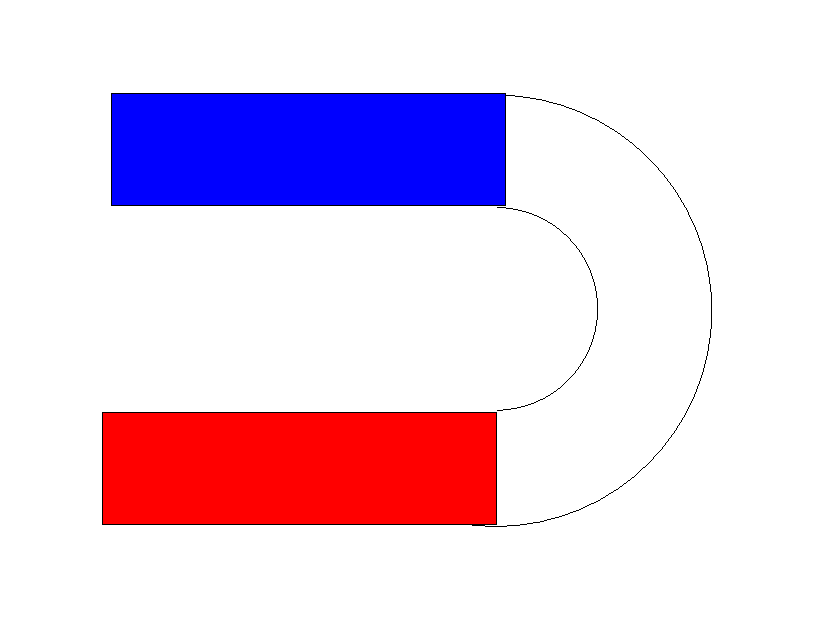
\includegraphics[scale=0.5]{img/horseshoe-magnet.eps}} \\
  \subfloat[“尾对尾”接在一起的列表]{\includegraphics[scale=0.5]{img/front-rear-queue.ps}}
  \caption{使用front列表和rear列表实现的队列形如一个马蹄形磁铁。} \label{fig:horseshoe-magnet}
\end{figure}

使用两个列表后,我们把新元素加入rear列表的头部,性能为常数时间;出队时,我们将元素从front列表的头部取走,性能也是常数时间。这样队列的性能要求就都可以满足了。

下面的Haskell代码定义了这种paired-list队列。

\lstset{language=Haskell}
\begin{lstlisting}
type Queue a = ([a], [a])

empty = ([], [])
\end{lstlisting}

令函数$front(Q)$和$rear(Q)$分别返回front和rear列表,函数$Queue(F, R)$从两个列表$F$和$R$构造一个队列。入队操作\textproc{EnQueue}(push)和出队\textproc{DeQueue}(pop)可以定义如下:

\be
push(Q, x) = Queue(front(Q), \{ x \} \cup rear(Q))
\ee

\be
pop(Q) = Queue(tail(front(Q)), rear(Q))
\ee

其中若列表$X =  \{ x_1, x_2, ..., x_n \}$,则函数$tail(X) = \{ x_2, x_3, ..., x_n \}$为除第一元素外的剩余元素列表。

但是,我们必须解决一个关键问题,经过一系列出队操作后,front列表有可能变空,而rear列表中还有元素。这时如果再进行出队操作将如何处理?一种方案是将rear列表反转后替换front列表。

为此,每次出队操作后,我们都执行一次平衡检查,即队列$Q$的front和rear列表分别为$F = front(Q)$和$R = fear(Q)$。

\be
balance(F, R) = \left \{
  \begin{array}
  {r@{\quad:\quad}l}
  Queue(reverse(R), \phi) & F = \phi \\
  Q & otherwise
  \end{array}
\right .
\ee

如果front列表不为空,无需任何额外处理;否则如果front列表变为空,就用反转的rear列表来代替,而新的rear列表为空。

这样改动后的入队和出队操作如下:

\be
push(Q, x) = balance(F, \{ x \} \cup R)
\ee

\be
pop(Q) = balance(tail(F), R)
\ee

下面完整的Haskell例子程序实现了上述算法。

\begin{lstlisting}
balance :: Queue a -> Queue a
balance ([], r) = (reverse r, [])
balance q = q

push :: Queue a -> a -> Queue a
push (f, r) x = balance (f, x:r)

pop :: Queue a -> Queue a
pop ([], _) = error "Empty"
pop (_:f, r) =  balance (f, r)
\end{lstlisting}

虽然我们仅仅在front和rear列表的头部进行入队和出队操作,但是性能并不能总保证为常数时间。
尽管如此,整体的分摊性能是可以达到常数时间的。将rear列表反转所需时间和列表长度成正比。
这一步的复杂度为$O(n)$,其中$n=|R|$。我们将分担性能的证明作为习题留给读者。

\subsection{Paired-array队列-一种对称实现}
\index{队列!Paired-array队列}

存在一个和paired-list队列对称的有趣实现。在某些老的编程语言中,例如旧版本的BASIC,只有数组可用,不能使用指针、或者结构等复合类型来定义链表。尽管可以使用一个额外的数组来记录索引,从而用数组实现链表。但是还存在更简单的方法来实现分摊性能为常数时间的队列。

下面的表比较了数组和链表,假设元素个数为$n$,各项操作的性能如下:

\begin{tabular}{l | c | r}
  \hline
  操作 & 数组 & 链表 \\
  \hline
  在头部加入 & $O(n)$ & $O(1)$ \\
  在尾部加入 & $O(1)$ & $O(n)$ \\
  在头部删除 & $O(n)$ & $O(1)$ \\
  在尾部删除 & $O(1)$ & $O(n)$ \\
  \hline
\end{tabular}

可以看到,链表在头部的性能为常数时间,而在尾部为线性时间;而数组在尾部操作为常数时间(简单起见,假设空间足够,无需申请),但是在头部操作为线性时间。这是因为需要准备或者消除一个空档需要将后继的元素依次移动(参见插入排序一章的介绍)。

上表给出了一个有趣的特性,我们可以利用它设计一个类似paired-list的解决方法:将两个数组“头对头”连接起来,形成一个马蹄形的队列,如图\ref{fig:horseshoe-array}所示。

\begin{figure}[htbp]
  \centering
  \subfloat[马蹄形磁铁]{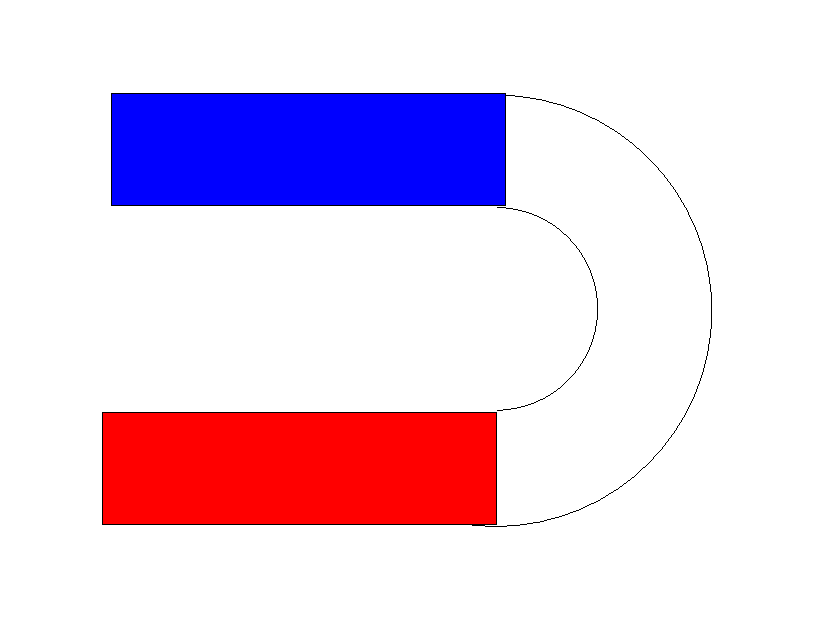
\includegraphics[scale=0.5]{img/horseshoe-magnet.eps}}
  \subfloat[将两个数组“头对头”连接起来]{\includegraphics[scale=0.5]{img/front-rear-array-queue.ps}}
  \caption{使用front数组和rear数组实现的队列形如一个马蹄形磁铁。} \label{fig:horseshoe-array}
\end{figure}

下面的Python例子程序定义了paired-array队列\footnote{我们省略了旧式BASIC代码。在Python中,实际是使用了内置的list而不是array。也可参考本书附带的C/C++例子程序,它们使用内置的数组来实现队列。}。

\lstset{language=Python}
\begin{lstlisting}
class Queue:
    def __init__(self):
        self.front = []
        self.rear = []

def is_empty(q):
    return q.front == [] and q.rear == []
\end{lstlisting}

相应的入队操作\textproc{Push}()和出队操作\textproc{Pop}()都仅在数组的尾部执行。

\begin{algorithmic}
\Function{Push}{$Q, x$}
  \State \textproc{Append}(\Call{Rear}{$Q$}, $x$)
\EndFunction
\end{algorithmic}

其中过程\textproc{Append}()将元素$x$加入到数组的尾部,并进行必要的内存申请。有多种内存处理策略,除了重新申请更大的内存,然后复制元素外,还可以设置内存上限,并在用满后报错。

\begin{algorithmic}
\Function{Pop}{$Q$}
  \If{\Call{Front}{$Q$} $= \phi$}
    \State \Call{Front}{$Q$} $\gets$ \textproc{Reverse}(\Call{Rear}{$Q$})
    \State \Call{Rear}{$Q$} $\gets \phi$
  \EndIf
  \State $N \gets$ \textproc{Length}(\Call{Front}{$Q$})
  \State $x \gets$ \Call{Front}{$Q$}[N]
  \State \textproc{Length}(\Call{Front}{$Q$}) $\gets N - 1$
  \State \Return $x$
\EndFunction
\end{algorithmic}

简单起见,在删除元素后,我们并未缩小数组的尺寸。可以通过检查数组的长度是否为0来判断front数组是否为空。这里跳过了这些细节。

下面的Python例子程序实现了入队和出队操作。

\begin{lstlisting}
def push(q, x):
    q.rear.append(x)

def pop(q):
    if q.front == []:
        q.rear.reverse()
        (q.front, q.rear) = (q.rear, [])
    return q.front.pop()
\end{lstlisting}

和paried-list队列类似,由于反转数组也是线性时间的,这一实现的分摊性能为常数时间$O(1)$。

\begin{Exercise}
\begin{itemize}
\item 证明paired-list队列的分摊性能为常数时间$O(1)$。
\item 证明paired-array队列的分摊性能为常数时间$O(1)$。
\end{itemize}
\end{Exercise}

% ================================================================
%                 Balanced Queue
% ================================================================
\section{小改进:平衡队列}
\index{队列!平衡队列}

虽然paired-list队列的入队和出队操作的分摊复杂度为常数时间$O(1)$,但是在最坏情况下的性能很差。例如front列表中只有一个元素,然后我们将$n$个元素连续加入队列,这里$n$是一个很大的整数。此时执行一次出队操作就会进入最坏情况。

根据设计规则,全部$n$个元素都加入了rear列表。执行一次弹出操作后,front列表变为空。于是开始反转rear列表,这一操作是线性时间$O(n)$的,和rear列表的长度成比例。某些场合下,当$n$很大时,这一时间消耗太大,无法满足要求。

造成这一最坏情况的原因是由于front和rear列表极不平衡。我们可以修改队列的设计来改进平衡性。例如加入一条平衡限制:

\be
  | R | \leq | F |
\label{eq:balance-invariant}
\ee

其中$R = Rear(Q)$,$F = Front(Q)$分别是队列中的前后两个列表。记号$|L|$表示列表$L$的长度。这一条件保证了rear列表的长度不小于front列表。当条件不满足时,就执行反转操作。

使用这一限制条件,需要频繁获取列表的长度。由于列表本质上是单向链表,因此需要线性时间来得到长度。我们可以将列表的长度缓存起来,并在增减元素时更新长度。这样就可以在常数时间获得列表长度。

下面的Haskell例子代码在paired-list队列的基础上增加了长度缓存信息。

\lstset{language=Haskell}
\begin{lstlisting}
data BalanceQueue a = BQ [a] Int [a] Int
\end{lstlisting}

只要保持式(\ref{eq:balance-invariant})一直得到满足,就可以通过检查front列表的长度来判断队列是否为空:

\be
  F = \phi \Leftrightarrow |F| = 0
\ee

本节余下的部份中们,我们一律认为可以在常数时间内获得列表$L$的长度$|L|$。

入队和出队操作基本和以前一样,我们需要额外传入列表的长度信息,检查平衡条件,如有必要就执行反转操作。

\be
  push(Q, x) = balance(F, |F|, \{ x \} \cup R, |R| + 1)
\ee

\be
  pop(Q) = balance(tail(F), |F|-1, R, |R|)
\ee

其中函数$balance()$定义如下:

\be
  balance(F, |F|, R, |R|) = \left \{
  \begin{array}
  {r@{\quad:\quad}l}
  Queue(F, |F|, R, |R|) & |R| \leq |F| \\
  Queue(F \cup reverse(R), |F| + |R|, \phi, 0) & otherwise
  \end{array}
\right .
\ee

这里函数$Queue()$接受四个参数:front列表和缓存的长度;rear列表和长度。这些信息用以构造一个paired-list队列。

下面的Haskell例子程序实现了平衡paired-list队列。程序使用了Haskell的类型系统来保证实现符合抽象队列的定义。

\lstset{language=Haskell}
\begin{lstlisting}
instance Queue BalanceQueue where
    empty = BQ [] 0 [] 0

    isEmpty (BQ _ lenf _ _) = lenf == 0

    -- Amortized O(1) time push
    push (BQ f lenf r lenr) x = balance f lenf (x:r) (lenr + 1)

    -- Amortized O(1) time pop
    pop (BQ (_:f) lenf r lenr) = balance f (lenf - 1) r lenr

    front (BQ (x:_) _ _ _) = x

balance f lenf r lenr
    | lenr <= lenf = BQ f lenf r lenr
    | otherwise = BQ (f ++ (reverse r)) (lenf + lenr) [] 0
\end{lstlisting}

\begin{Exercise}
选择一门命令式语言,实现平衡paired-array队列。
\end{Exercise}

% ================================================================
%                 Realtime Queue
% ================================================================
\section{进一步改进:实时队列}
\index{队列!实时队列}

改善平衡性后虽然可以避免最差情况,但是反转rear列表的的性能仍然是$O(n)$的,其中$n = |R|$。尽管分摊性能为常数时间,但如果rear列表很长,某次操作的性能仍然会很差。在某些实时系统中,我们必须保证在最坏情况下的性能也达到要求。

根据前面的分析,计算的瓶颈在$ F \cup reverse(R)$,当$|R| > |F|$时会发生这一操作。考虑$|F|$和$|R|$都是整数,发生这一操作时,我们有:

\be
  |R| = |F| + 1
\ee

$F$和$reverse(R)$的结果都是单向链表,链结它们耗时$O(|F|)$,此外还需要$O(|R|)$时间反转rear列表,因此总时间为$O(n)$,其中$n = |F| + |R|$。也就是说,和队列中的元素个数成正比。

为了实现实时队列,我们不能一次性计算$ F \cup reverse(R)$。解决策略是将这一耗时的计算分派到各次入队和出队操作中去。这样虽然单次的入队和出队需要做的事情多了,但是可以避免最坏情况下性能退化为线性时间。

\subsubsection{逐步反转}
\index{队列!逐步反转}

我们首先分析一下典型的函数式反转算法。

\be
  reverse(X) = \left \{
  \begin{array}
  {r@{\quad:\quad}l}
  \phi & X = \phi \\
  reverse(X') \cup \{ x_1 \} & otherwise
  \end{array}
\right .
\ee

其中$X' = tail(X) = \{ x_2, x_3, ...\}$。

若列表为空,则反转结果也是一个空列表。否则,我们取出第一个元素$x_1$,将剩余元素$\{x_2, x_3, ..., x_n \}$反转为$\{x_n, x_{n-1}, .., x_3, x_2 \}$,然后在将$x_1$追加到末尾。

但是,这一算法的性能不佳,追加元素到末尾用时和列表长度成正比。因此这一反转操作的性能为$O(n^2)$。

另外一种实现方式是使用\underline{尾递归}:

\be
  reverse(X) = reverse'(X, \phi)
\ee

其中

\be
 reverse'(X, A) = \left \{
  \begin{array}
  {r@{\quad:\quad}l}
  A & X = \phi \\
  reverse'(X', \{ x_1 \} \cup A) & otherwise
  \end{array}
\right .
\ee

我们称$A$为\underline{accumulator},它不断累积中间结果。任何时候,当调用$reverse'(X, A)$时,$X$包含尚未反转的元素,$A$包含迄今为止反转完的元素。当第$i$次调用$reverse'()$时,$X$和$A$分别包含如下内容:

\[
  \begin{array}{r@{\quad}l}
  X = \{x_i, x_{i+1}, ..., x_n \} & A = \{ x_{i-1}, x_{i-2}, ... x_1 \}
  \end{array}
\]

每次递归,如果不是边界情况,我们用常数时间从$X$取出第一个元素;然后将其链结到$A$的前面,这一步同样仅耗时常数时间$O(1)$。同样的操作重复$n$次,因此这一反转算法时线性时间$O(n)$的。

尾递归\cite{tail-call}\cite {recursion}算法可以很容易从一次性计算改为逐步计算。整体过程相当于一系列的状态转换。我们定义一个状态机,包含两种状态:反转状态$S_r$表示正在进行反转(未完成);完成状态$S_f$表示反转已经结束(完成)。下面的Haskell例子程序将状态定义为类型。

\lstset{language=Haskell}
\begin{lstlisting}
data State a = | Reverse [a] [a]
               | Done [a]
\end{lstlisting}

使用这两种状态,我们可以调度(slow-down)函数$reverse'(X, A)$的计算。

\be
  step(S, X, A) = \left \{
  \begin{array}
  {r@{\quad:\quad}l}
  (S_f, A) & S = S_r \land X = \phi \\
  (S_r, X', \{ x_1 \} \cup A) & S = S_r \land X \neq \phi \\
  \end{array}
\right .
\ee

每一步,我们先检查当前的状态,如果状态为$S_r$(反转中),但是$X$中已没有剩余元素需要反转,就将状态变换为完成$S_f$;否则,我们取出$X$中的第一个元素,将其链结到$A$的前面,接下来与之前不同,我们不再进行递归调用,这一步计算到此结束。当前的状态,以及反转的中间步骤结果$X$和$A$被保存下来,我们可以在以后的任何时候使用这些内容,再调用$step$函数继续反转。

下面是逐步反转的一个例子:

\[
\begin{array}{lcl}
step(S_r, "hello", \phi) & = & (S_r, "ello", "h") \\
step(S_r, "ello", "h") & = & (S_r, "llo", "eh") \\
... & & \\
step(S_r, "o", "lleh") & = & (S_r, \phi, "olleh") \\
step(S_r, \phi, "olleh") & = & (S_f, "olleh")
\end{array}
\]

下面的Haskell代码描述了同样的例子:

\lstset{language=Haskell}
\begin{lstlisting}
step $ Reverse "hello" [] = Reverse "ello" "h"
step $ Reverse "ello" "h" = Reverse "llo" "eh"
...
step $ Reverse "o" "lleh" = Reverse [] "olleh"
step $ Reverse [] "olleh" = Done "olleh"
\end{lstlisting}

现在我们可以将反转计算逐步分散到入队和出队操作中。但是这仅解决了一半问题。我们需要逐步分解$ F \cup reverse(R)$计算。因此接下来需要调度(slow-down)列表的连接操作$F \cup ..$。连接操作的复杂度为$O(|F|)$。同样,我们的目标是将它分散到入队和出队操作中去。

\subsubsection{逐步连接}
\index{队列!逐步连接}

实现列表的逐步连接要比逐步反转难度更大。我们可以利用逐步反转的结果。这里有一个小技巧:为了实现$X \cup Y$,我们可以先将$X$反转为$\overleftarrow{X}$,然后逐一将$\overleftarrow{X}$中的元素取出,放到$Y$的前面。这和我们前面实现的$reverse'$类似。

\be
  \begin{array}{rcl}
    X \cup Y & \equiv & reverse(reverse(X)) \cup Y \\
             & \equiv & reverse'(reverse(X), \phi) \cup Y \\
             & \equiv & reverse'(reverse(X), Y) \\
             & \equiv & reverse'(\overleftarrow{X}, Y)
  \end{array}
\ee

这一事实表明,我们可以增加另一个状态来控制$step()$函数,在$R$反转后,逐步操作$\overleftarrow{F}$实现连接。

整个操作被分解为两个阶段:

\begin{enumerate}
\item 同时反转$F$和$R$,逐步得到$\overleftarrow{F} = reverse(F)$和$\overleftarrow{R} = reverse(R)$;
\item 逐步从$\overleftarrow{F}$取出元素,链接到$\overleftarrow{R}$前面。
$\overleftarrow{R}$.
\end{enumerate}

为此我们定义三种状态:$S_r$代表反转;$S_c$代表连接;$S_f$代表完成。

下面的Haskell例子程序定义了这三种状态。

\lstset{language=Haskell}
\begin{lstlisting}
data State a = Reverse [a] [a] [a] [a]
             | Concat [a] [a]
             | Done [a]
\end{lstlisting}

由于我们同时反转$F$和$R$,因此反转状态变量带有一对列表和一对accumulator。

状态转换按照两个阶段测策略进行定义。记$F = \{ f_1, f_2, ... \}$、$F' = tail(F) = \{f_2, f_3, ... \}$、
$R = \{ r_1, r_2, ... \}$、$R' = tail(R) = \{ r_2, r_3, ... \}$。一个状态$\mathcal{S}$包含它的类型$S$,可以是$S_r$、$S_c$和$S_f$的一种。同时状态$\mathcal{S}$中还包含必要的参数,如$F$、$\overleftarrow{F}$、$X$、$A$等作为中间结果。状态不同,包含的参数也有所不同。

\be
  next(\mathcal{S}) = \left \{
  \begin{array}
  {r@{\quad:\quad}l}
  (S_r, F', \{ f_1 \} \cup \overleftarrow{F}, R', \{ r_1 \} \cup \overleftarrow{R}) & S = S_r \land F \neq \phi \land R \neq \phi \\
  (S_c, \overleftarrow{F}, \{ r_1 \} \cup \overleftarrow{R}) & S = S_r \land F = \phi \land R = \{ r_1 \} \\
  (S_f, A) & S = S_c \land X = \phi \\
  (S_c, X', \{ x_1 \} \cup A) & S = S_c \land X \neq \phi
  \end{array}
\right .
\ee

相应的Haskell程序如下:

\lstset{language=Haskell}
\begin{lstlisting}
next (Reverse (x:f) f' (y:r) r') = Reverse f (x:f') r (y:r')
next (Reverse [] f' [y] r') = Concat f' (y:r')
next (Concat 0 _ acc) = Done acc
next (Concat (x:f') acc) = Concat f' (x:acc)
\end{lstlisting}

接下来我们需要将这些递进的步骤分配到每个出队和入队操作中以实现一个实时$O(1)$的纯函数式队列。

\subsubsection{汇总}

在给出最终的实时队列实现前,我们先来分析一下为了计算$F \cup reverse(R)$,总共需要多少递进步骤。根据平衡队列的条件,有$|R| = |F| + 1$。记$M = |F|$。

由于某次出队或入队操作造成队列不平衡时,我们开始逐步计算$F \cup reverse(R)$。总共需要$M+1$步来反转$R$,我们同时在这些步骤内完成了对$F$的反转。此后,我们需要再用$M+1$步来进行连接操作。因此总共花费了$2M+2$步。

最直观的想法是在每一个出队和入队操作中分配一个递进步骤。但是我们需要回答一个关键问题:在我们完成$2M+2$步操作之前,队列有没有可能由于接下来的一系列入队和出队操作,再次变得不平衡?

关于这一问题有两个事实,一个是好消息,一个是坏消息。

我们先看好消息。很幸运,在我们花费$2M+2$步操作计算$F \cup reverse(R)$完成之前,连续的入队操作不可能再次使得队列变得不平衡。因为一旦开始恢复平衡的处理,经过$2M+2$步后,我们就得到了一个新的front列表$F' = F \cup reverse(R)$。而下一次队列变得不平衡时,我们有:

\be
  \begin{array}{rcl}
  |R'| & = & |F'| + 1 \\
       & = & |F| + |R| + 1 \\
       & = & 2M + 2
  \end{array}
\ee

也就是说,从上次队列不平衡的时刻算起,即使我们不断持续将新元素入队,以最快的速度再次使得队列不平衡时,$2M+2$步计算恰好已经完成了。此时新的front列表被计算出来。我们可以安全地继续计算$F' \cup reverse(R')$。多亏了前面给出的平衡invariant,帮助我们保证了这一点。

但是还有一个坏消息。在$2M+2$步计算完成前,出队操作可能随时发生。这会产生一个尴尬的情况:我们需要从front列表取出元素,但是新的front列表$F' = F \cup reverse(R)$尚未计算好。此时没有一个可用的front列表。

一种解决方法是在第一阶段计算$reverse(F)$时,另外保存一份此前的front列表$F$。这样即使连续进行$M$次出队操作,我们仍然是安全的。表(\ref{tab:pop-before-m})给出了第一阶段逐步计算(同时反转$F$和$R$)的某个时刻队列的样子\footnote{有人会产生疑问,通常复制一个列表需要花费和列表长度成比例的线性时间。这样整个方案就有问题了。实际上,这一线性时间的列表复制根本不会发生。因为在纯函数式的环境下,出队或反转并不“修改”front列表。但是,如果尝试用paired数组实现一个对称解,并且in-place地修改数组,这一问题就会产生影响。为此,我们需要实现某种lazy复制,真正的复制操作并不立即发生,而是在每次反转的递进步骤中一步复制一个元素。具体的实现留给读者作为练习}。

\begin{table}
\centering
\begin{tabular}{l l l}
  保存的front列表 & 进行中的计算 & 新的rear列表 \\
  \hline
  $\{ f_i, f_{i+1}, ..., f_M \}$ & $(S_r, \tilde{F}, ..., \tilde{R}, ...)$ & $ \{ ... \}$ \\
  前$i-1$个元素已出队 & $\overleftarrow{F}$和$\overleftarrow{R}$的中间结果 & 包含新入队的元素
\end{tabular}
\caption{前$M$步完成前的队列中间状态。}
\label{tab:pop-before-m}
\end{table}

经过$M$次出队操作,$F$的副本已经用光。我们此时刚刚开始进逐步连接的计算阶段。此时如果继续进行出队操作会怎样?

事实上,由于$F$的副本被用光(变成了$phi$),我们无需再进行连接操作了。这是因为$F \cup \overleftarrow{R} = \phi \cup \overleftarrow{R} = \overleftarrow{R}$。

这一点告诉我们,在进行连接操作时,我们只需要将$F$中尚未出队的元素连接起来。因为元素从$F$的头部逐一出队,我们可以使用一个计数器(counter)来记录$F$中剩余元素的个数。当开始计算$F \cup reverse(R)$时,计数器为0,每次反转$F$中的一个元素时,就将计数器加一,表示将来我们需要连接这个元素;每次出队操作,就将计数器减一,表示我们将来可以少连接一个元素。显然在连接操作的每步中,我们也需要递减计数器。当且仅当计数器为0的时候,我们无需继续进行连接操作。

根据以上的分析,我们可以给出纯函数式的实时队列的完整实现了。为了简化状态转换,我们可以增加一个idle状态$S_0$。下面的Haskell例子程序给出了这一修改过的状态定义。

\lstset{language=Haskell}
\begin{lstlisting}
data State a = Empty
             | Reverse Int [a] [a] [a] [a] -- n, f', acc_f' r, acc_r
             | Append Int [a] [a]          -- n, rev_f', acc
             | Done [a] -- result: f ++ reverse r
\end{lstlisting}

队列的数据结构分为三个部分:front列表(带有长度信息);正在计算中的$F \cup reverse(R)$的中间状态;和rear列表(带有长度信息)。

下面的Haskell例子程序定义了实时队列的数据结构。

\lstset{language=Haskell}
\begin{lstlisting}
data RealtimeQueue a = RTQ [a] Int (State a) [a] Int
\end{lstlisting}

空队列包含空的front和rear列表,以及一个idle状态$S_0$,记为$Queue(\phi, 0, S_0, \phi, 0)$。根据平衡invariant的定义,我们可以通过检查$|F|=0$与否来判断一个队列是否为空。入队和出队操作修改如下:

\be
  push(Q, x) = balance(F, |F|, \mathcal{S}, \{ x \} \cup R, |R|+1)
\ee

\be
  pop(Q) = balance(F', |F|-1, abort(\mathcal{S}), R, |R|)
\ee

最大的变化在于$abort()$函数。根据前面的分析,在出队时我们递减计数器,这样将来可以少连接一个元素。我们将其定义为aborting。我们稍后介绍它的具体实现。

相应的Haskell出队和入队操作可以由下面的例子程序给出。

\lstset{language=Haskell}
\begin{lstlisting}
push (RTQ f lenf s r lenr) x = balance f lenf s (x:r) (lenr + 1)
pop (RTQ (_:f) lenf s r lenr) = balance f (lenf - 1) (abort s) r lenr
\end{lstlisting}

函数$balance()$首先检查平衡invariant,如果违反了,我们需要启动$F \cup reverse(R)$的逐步计算来恢复平衡;否则,我们仅仅执行异步尚未完成的递进计算。

\be
  balance(F, |F|, \mathcal{S}, R, |R|) = \left \{
  \begin{array}
  {r@{\quad:\quad}l}
  step(F, |F|, \mathcal{S}, R, |R|) & |R| \leq |F| \\
  step(F, |F| + |R|, (S_r, 0, F, \phi, R, \phi) \phi, 0) & otherwise
  \end{array}
\right .
\ee

相应的Haskell例子程序如下:

\lstset{language=Haskell}
\begin{lstlisting}
balance f lenf s r lenr
    | lenr <= lenf =  step f lenf s r lenr
    | otherwise = step f (lenf + lenr) (Reverse 0 f [] r []) [] 0
\end{lstlisting}

函数$step()$将状态机转换到下一个状态,全部递进计算结束后,状态转换到idle状态$S_0$。

\be
  step(F, |F|, \mathcal{S}, R, |R|) = \left \{
  \begin{array}
  {r@{\quad:\quad}l}
  Queue(F', |F|, S_0, R, |R|) &  S' = S_f \\
  Queue(F, |F|, \mathcal{S}', R, |R|) & otherwise
  \end{array}
  \right .
\ee

Where $\mathcal{S}' = next(\mathcal{S})$ is the next state transferred;
$F' = F \cup reverse(R)$, is the final new front list result from the incremental
computing. The real
state transferring is implemented in $next()$ function as the following. It's different
from previous version by adding the counter field $n$ to record how many elements left
we need to concatenate.

\be
  next(\mathcal{S}) = \left \{
  \begin{array}
  {r@{\quad:\quad}l}
  (S_r, n+1, F', \{ f_1 \} \cup \overleftarrow{F}, R', \{ r_1 \} \cup \overleftarrow{R}) &
      S = S_r \land F \neq \phi \\
  (S_c, n, \overleftarrow{F}, \{ r_1 \} \cup \overleftarrow{R}) &
      S = S_r \land F = \phi \\
  (S_f, A) & S = S_c \land n = 0 \\
  (S_c, n-1, X', \{ x_1 \} \cup A) & S = S_c \land n \neq 0 \\
  \mathcal{S} & otherwise
  \end{array}
\right .
\ee

And the corresponding Haskell code is like this.

\lstset{language=Haskell}
\begin{lstlisting}
next (Reverse n (x:f) f' (y:r) r') = Reverse (n+1) f (x:f') r (y:r')
next (Reverse n [] f' [y] r') = Concat n f' (y:r')
next (Concat 0 _ acc) = Done acc
next (Concat n (x:f') acc) = Concat (n-1) f' (x:acc)
next s = s
\end{lstlisting}

Function $abort()$ is used to tell the state machine, we can concatenate one element
less since it is popped.

\be
  abort(\mathcal{S}) = \left \{
  \begin{array}
  {r@{\quad:\quad}l}
  (S_f, A') & S = S_c \land n = 0 \\
  (S_c, n-1, X' A) & S = S_c \land n \neq 0 \\
  (S_r, n-1, F, \overleftarrow{F}, R, \overleftarrow{R}) & S = S_r \\
  \mathcal{S} & otherwise
  \end{array}
\right .
\ee

Note that when $n = 0$ we actually rollback one concatenated element by
return $A'$ as the result but not $A$. (Why? this is left as an exercise.)

The Haskell code for abort function is like the following.

\lstset{language=Haskell}
\begin{lstlisting}
abort (Concat 0 _ (_:acc)) = Done acc -- Note! we rollback 1 elem
abort (Concat n f' acc) = Concat (n-1) f' acc
abort (Reverse n f f' r r') = Reverse (n-1) f f' r r'
abort s = s
\end{lstlisting}

It seems that we've done, however, there is still one tricky issue hidden
behind us.
If we push an element $x$ to an empty queue, the result queue will be:
\[
  Queue(\phi, 1, (S_c, 0, \phi, \{ x \}), \phi, 0)
\]

If we perform pop immediately, we'll get an error! We found that
the front list is empty although the previous computation of $F \cup reverse(R)$
has been finished. This is because it takes one more extra step to
transfer from the state $(S_c, 0, \phi, A)$ to $(S_f, A)$. It's necessary
to refine the $\mathcal{S}'$ in $step()$ function a bit.

\be
  \mathcal{S}' = \left \{
  \begin{array}
  {r@{\quad:\quad}l}
  next(next(\mathcal{S})) & F = \phi \\
  next(\mathcal{S}) & otherwise
  \end{array}
\right .
\ee

The modification reflects to the below Haskell code:

\lstset{language=Haskell}
\begin{lstlisting}
step f lenf s r lenr =
    case s' of
      Done f' -> RTQ f' lenf Empty r lenr
      s' -> RTQ f lenf s' r lenr
    where s' = if null f then next $ next s else next s
\end{lstlisting} %$

Note that this algorithm differs from the one given by Chris Okasaki in \cite{okasaki-book}.
Okasaki's algorithm executes two steps per pop and push, while the one presents in
this chapter executes only one per pop and push, which leads to more distributed
performance.

\begin{Exercise}
\begin{itemize}
\item Why need we rollback one element when $n=0$ in $abort()$ function?

\item Realize the real-time queue with symmetric paired-array queue solution in your favorite
imperative programming language.

\item In the footnote, we mentioned that when we start incremental reversing
with in-place paired-array solution, copying the array can't be done monolithic
or it will lead to linear time operation. Implement the lazy copying
so that we copy one element per step along with the reversing.

\end{itemize}
\end{Exercise}


% ================================================================
%                 Lazy Real-time queue
% ================================================================
\section{Lazy real-time queue}
\index{Queue!Lazy real-time queue}

The key to realize a real-time queue is to break down the expensive
$F \cup reverse(R)$ to avoid monolithic computation. Lazy evaluation
is particularly helpful in such case. In this section, we'll explore
if there is some more elegant solution by exploit laziness.

Suppose that there exits a function $rotate()$,
which can compute $F \cup reverse(R)$ incrementally. that's to say,
with some accumulator $A$, the following two functions are equivalent.

\be
  rotate(X, Y, A) \equiv X \cup reverse(Y) \cup A
  \label{eq:rot-def}
\ee

Where we initialized $X$ as the front list $F$, $Y$ as the rear list $R$,
and the accumulator $A$ is initialized as empty $\phi$.

The trigger of rotation is still as same as before when $|F| + 1 = |R|$.
Let's keep this constraint as an invariant during the whole rotation process,
that $|X| + 1 = |Y|$ always holds.

It's obvious to deduce to the trivial case:

\be
  rotate(\phi, \{ y_1 \}, A) = \{ y_1 \} \cup A
\ee

Denote $X = \{ x_1, x_2, ... \}$, $Y = \{ y_1, y_2, ...\}$, and
$X' = \{ x_2, x_3, ...  \}$, $Y' = \{ y_2, y_3, ...\}$ are the rest
of the lists without the first element for $X$ and $Y$ respectively.
The recursion case is ruled out as the following.

\be
  \begin{array}{rcll}
  rotate( X, Y, A ) & \equiv & X \cup reverse(Y) \cup A & \mbox{Definition of (}\ref{eq:rot-def} \mbox{)} \\
  & \equiv & \{ x_1 \} \cup (X' \cup reverse(Y) \cup A) & \mbox{Associative of } \cup \\
  & \equiv & \{ x_1 \} \cup (X' \cup reverse(Y') \cup (\{ y_1 \} \cup A)) & \mbox{Nature of reverse and associative of }  \cup \\
  & \equiv & \{ x_1 \} \cup rotate(X', Y', \{ y_1 \} \cup A) & \mbox{Definition of (} \ref{eq:rot-def} \mbox{)}
  \end{array}
\ee

Summarize the above two cases, yields the final incremental rotate algorithm.

\be
rotate(X, Y, A) = \left \{
  \begin{array}
  {r@{\quad:\quad}l}
  \{ y_1 \} \cup A & X = \phi \\
  \{ x_1 \} \cup rotate(X', Y', \{ y_1 \} \cup A) & otherwise
  \end{array}
\right .
\ee

If we execute $\cup$ lazily instead of strictly, that is, execute $\cup$
once pop or push operation is performed, the computation of $rotate$ can
be distribute to push and pop naturally.

Based on this idea, we modify the paired-list queue definition to change
the front list to a lazy list, and augment it with a computation stream.
\cite{SICP}. When the queue triggers re-balance constraint by some
pop/push, that
$|F| + 1 = |R|$, The algorithm creates a lazy rotation computation,
then use this lazy rotation as the new front list $F'$; the new rear
list becomes $\phi$, and a copy of $F'$ is maintained as a stream.

After that, when we performs every push and pop; we consume the
stream by forcing a $\cup$ operation. This results us advancing one
step along the stream, $ \{ x \} \cup F''$, where $F' = tail(F')$.
We can discard $x$, and replace the stream $F'$ with $F''$.

Once all of the stream is exhausted, we can start another rotation.

In order to illustrate this idea clearly, we turns to Scheme/Lisp
programming language to show example codes, because it gives us
explicit control of laziness.

In Scheme/Lisp, we have the following three tools to deal with lazy
stream.

\lstset{language=Lisp}
\begin{lstlisting}
(define (cons-stream a b) (cons a (delay b)))

(define stream-car car)

(define (stream-cdr s) (cdr (force s)))
\end{lstlisting}

So 'cons-stream' constructs a 'lazy' list from an element $x$
and an existing list $L$ without really evaluating
the value of $L$; The evaluation is actually delayed to
'stream-cdr', where the computation is forced. delaying can
be realized by lambda calculus, please refer to \cite{SICP} for
detail.

The lazy paired-list queue is defined as the following.

\lstset{language=Lisp}
\begin{lstlisting}
(define (make-queue f r s)
  (list f r s))

;; Auxiliary functions
(define (front-lst q) (car q))

(define (rear-lst q) (cadr q))

(define (rots q) (caddr q))
\end{lstlisting}

A queue is consist of three parts, a front list, a rear list,
and a stream which represents the computation of $F \cup reverse(R)$.
Create an empty queue is trivial as making all these three parts
null.

\begin{lstlisting}
(define empty (make-queue '() '() '()))
\end{lstlisting}

Note that the front-list is also lazy stream actually, so we need use
stream related functions to manipulate it. For example, the following
function test if the queue is empty by checking the front lazy list stream.

\begin{lstlisting}
(define (empty? q) (stream-null? (front-lst q)))
\end{lstlisting}

The push function is almost as same as the one given in previous section.
That we put the new element in front of the rear list; and then examine
the balance invariant and do necessary balancing works.

\be
push(Q, x) = balance(\mathcal{F}, \{ x \} \cup R, \mathcal{R}_s)
\ee

Where $\mathcal{R}$ represents the lazy stream of front list; $\mathcal{R}_s$ is
the stream of rotation computation. The relative Scheme/Lisp
code is give below.

\begin{lstlisting}
(define (push q x)
  (balance (front-lst q) (cons x (rear q)) (rots q)))
\end{lstlisting}

While pop is a bit different, because the front list is actually lazy stream,
we need force an evaluation. All the others are as same as before.

\be
pop(Q) = balance(\mathcal{F}', R, \mathcal{R}_s)
\ee

Here $\mathcal{F}'$, force one evaluation to $\mathcal{F}$, the Scheme/Lisp
code regarding to this equation is as the following.

\begin{lstlisting}
(define (pop q)
  (balance (stream-cdr (front-lst q)) (rear q) (rots q)))
\end{lstlisting}

For illustration purpose, we skip the error handling (such as pop from
an empty queue etc) here.

And one can access the top element in the queue by extract from
the front list stream.

\begin{lstlisting}
(define (front q) (stream-car (front-lst q)))
\end{lstlisting}

The balance function first checks if the computation stream is completely
exhausted, and starts new rotation accordingly; otherwise, it just consumes
one evaluation by enforcing the lazy stream.

\be
balance(Q) = \left \{
  \begin{array}
  {r@{\quad:\quad}l}
  Queue(\mathcal{F}', \phi, \mathcal{F}') & \mathcal{R}_s = \phi \\
  Queue(\mathcal{F}, R, \mathcal{R}_s') & otherwise
  \end{array}
\right .
\ee

Here $\mathcal{F}'$ is defined to start a new rotation.

\be
  \mathcal{F}' = rotate(F, R, \phi)
\ee

The relative Scheme/Lisp program is listed accordingly.

\begin{lstlisting}
(define (balance f r s)
  (if (stream-null? s)
      (let ((newf (rotate f r '())))
    (make-queue newf '() newf))
      (make-queue f r (stream-cdr s))))
\end{lstlisting}

The implementation of incremental rotate function is just as same as
what we analyzed above.

\begin{lstlisting}
(define (rotate xs ys acc)
  (if (stream-null? xs)
      (cons-stream (car ys) acc)
      (cons-stream (stream-car xs)
           (rotate (stream-cdr xs) (cdr ys)
               (cons-stream (car ys) acc)))))
\end{lstlisting}

We used explicit lazy evaluation in Scheme/Lisp. Actually, this program
can be very short by using lazy programming languages, for example,
Haskell.

\lstset{language=Haskell}
\begin{lstlisting}
data LazyRTQueue a = LQ [a] [a] [a] -- front, rear, f ++ reverse r

instance Queue LazyRTQueue where
    empty = LQ [] [] []

    isEmpty (LQ f _ _) = null f

    -- O(1) time push
    push (LQ f r rot) x = balance f (x:r) rot

    -- O(1) time pop
    pop (LQ (_:f) r rot) = balance f r rot

    front (LQ (x:_) _ _) = x

balance f r [] = let f' = rotate f r [] in LQ f' [] f'
balance f r (_:rot) = LQ f r rot

rotate [] [y] acc = y:acc
rotate (x:xs) (y:ys) acc = x : rotate xs ys (y:acc)
\end{lstlisting}

% ================================================================
%                 Short summary
% ================================================================
\section{Notes and short summary}
Just as mentioned in the beginning of this book in the first chapter,
queue isn't so simple as it was thought. We've tries to explain
algorithms and data structures both in imperative and in function
approaches; Sometimes, it gives impression that functional way is
simpler and more expressive in most time. However, there are still
plenty of areas, that more studies and works are needed to give equivalent
functional solution. Queue is such an important topic, that it
links to many fundamental purely functional data structures.

That's why Chris Okasaki made intensively study and took a great
amount of discussions in \cite{okasaki-book}. With purely functional
queue solved, we can easily implement dequeue with the similar
approach revealed in this chapter. As we can handle elements effectively
in both head and tail, we can advance one step ahead to realize
sequence data structures, which support fast concatenate, and
finally we can realize random access data structures to mimic
array in imperative settings. The details will be explained
in later chapters.

Note that, although we haven't mentioned priority queue, it's quite
possible to realized it with heaps. We have covered topic of heaps
in several previous chapters.

\begin{Exercise}
\begin{itemize}
\item Realize dequeue, wich support adding and removing elements on both sides in
constant $O(1)$ time in purely functional way.
\item Realize dequeue in a symmetric solution only with array in your
favorite imperative programming language.
\end{itemize}
\end{Exercise}

% ================================================================
%                 Appendix
% ================================================================

\begin{thebibliography}{99}

\bibitem{PODC96}
Maged M. Michael and Michael L. Scott. ``Simple, Fast, and Practical Non-Blocking and Blocking Concurrent Queue Algorithms''. http://www.cs.rochester.edu/research/synchronization/pseudocode/queues.html

\bibitem{SutterDDJ}
Herb Sutter. ``Writing a Generalized Concurrent Queue''. Dr. Dobb's Oct 29, 2008. http://drdobbs.com/cpp/211601363?pgno=1

\bibitem{CLRS}
Thomas H. Cormen, Charles E. Leiserson, Ronald L. Rivest and Clifford Stein. ``Introduction to Algorithms, Second Edition''. The MIT Press, 2001. ISBN: 0262032937.

\bibitem{okasaki-book}
Chris Okasaki. ``Purely Functional Data Structures''. Cambridge university press, (July 1, 1999), ISBN-13: 978-0521663502

\bibitem{tail-call}
Wikipedia. ``Tail-call''. http://en.wikipedia.org/wiki/Tail\_call

\bibitem{recursion}
Wikipedia. ``Recursion (computer science)''. http://en.wikipedia.org/wiki/Recursion\_(computer\_science)\#Tail-recursive\_functions

\bibitem{SICP}
Harold Abelson, Gerald Jay Sussman, Julie Sussman. ``Structure and Interpretation of Computer Programs, 2nd Edition''. MIT Press, 1996, ISBN 0-262-51087-1

\end{thebibliography}

\ifx\wholebook\relax \else
\end{document}
\fi
